\documentclass[1p]{elsarticle_modified}
%\bibliographystyle{elsarticle-num}

%\usepackage[colorlinks]{hyperref}
%\usepackage{abbrmath_seonhwa} %\Abb, \Ascr, \Acal ,\Abf, \Afrak
\usepackage{amsfonts}
\usepackage{amssymb}
\usepackage{amsmath}
\usepackage{amsthm}
\usepackage{scalefnt}
\usepackage{amsbsy}
\usepackage{kotex}
\usepackage{caption}
\usepackage{subfig}
\usepackage{color}
\usepackage{graphicx}
\usepackage{xcolor} %% white, black, red, green, blue, cyan, magenta, yellow
\usepackage{float}
\usepackage{setspace}
\usepackage{hyperref}

\usepackage{tikz}
\usetikzlibrary{arrows}

\usepackage{multirow}
\usepackage{array} % fixed length table
\usepackage{hhline}

%%%%%%%%%%%%%%%%%%%%%
\makeatletter
\renewcommand*\env@matrix[1][\arraystretch]{%
	\edef\arraystretch{#1}%
	\hskip -\arraycolsep
	\let\@ifnextchar\new@ifnextchar
	\array{*\c@MaxMatrixCols c}}
\makeatother %https://tex.stackexchange.com/questions/14071/how-can-i-increase-the-line-spacing-in-a-matrix
%%%%%%%%%%%%%%%

\usepackage[normalem]{ulem}

\newcommand{\msout}[1]{\ifmmode\text{\sout{\ensuremath{#1}}}\else\sout{#1}\fi}
%SOURCE: \msout is \stkout macro in https://tex.stackexchange.com/questions/20609/strikeout-in-math-mode

\newcommand{\cancel}[1]{
	\ifmmode
	{\color{red}\msout{#1}}
	\else
	{\color{red}\sout{#1}}
	\fi
}

\newcommand{\add}[1]{
	{\color{blue}\uwave{#1}}
}

\newcommand{\replace}[2]{
	\ifmmode
	{\color{red}\msout{#1}}{\color{blue}\uwave{#2}}
	\else
	{\color{red}\sout{#1}}{\color{blue}\uwave{#2}}
	\fi
}

\newcommand{\Sol}{\mathcal{S}} %segment
\newcommand{\D}{D} %diagram
\newcommand{\A}{\mathcal{A}} %arc


%%%%%%%%%%%%%%%%%%%%%%%%%%%%%5 test

\def\sl{\operatorname{\textup{SL}}(2,\Cbb)}
\def\psl{\operatorname{\textup{PSL}}(2,\Cbb)}
\def\quan{\mkern 1mu \triangleright \mkern 1mu}

\theoremstyle{definition}
\newtheorem{thm}{Theorem}[section]
\newtheorem{prop}[thm]{Proposition}
\newtheorem{lem}[thm]{Lemma}
\newtheorem{ques}[thm]{Question}
\newtheorem{cor}[thm]{Corollary}
\newtheorem{defn}[thm]{Definition}
\newtheorem{exam}[thm]{Example}
\newtheorem{rmk}[thm]{Remark}
\newtheorem{alg}[thm]{Algorithm}

\newcommand{\I}{\sqrt{-1}}
\begin{document}

%\begin{frontmatter}
%
%\title{Boundary parabolic representations of knots up to 8 crossings}
%
%%% Group authors per affiliation:
%\author{Yunhi Cho} 
%\address{Department of Mathematics, University of Seoul, Seoul, Korea}
%\ead{yhcho@uos.ac.kr}
%
%
%\author{Seonhwa Kim} %\fnref{s_kim}}
%\address{Center for Geometry and Physics, Institute for Basic Science, Pohang, 37673, Korea}
%\ead{ryeona17@ibs.re.kr}
%
%\author{Hyuk Kim}
%\address{Department of Mathematical Sciences, Seoul National University, Seoul 08826, Korea}
%\ead{hyukkim@snu.ac.kr}
%
%\author{Seokbeom Yoon}
%\address{Department of Mathematical Sciences, Seoul National University, Seoul, 08826,  Korea}
%\ead{sbyoon15@snu.ac.kr}
%
%\begin{abstract}
%We find all boundary parabolic representation of knots up to 8 crossings.
%
%\end{abstract}
%\begin{keyword}
%    \MSC[2010] 57M25 
%\end{keyword}
%
%\end{frontmatter}

%\linenumbers
%\tableofcontents
%
\newcommand\colored[1]{\textcolor{white}{\rule[-0.35ex]{0.8em}{1.4ex}}\kern-0.8em\color{red} #1}%
%\newcommand\colored[1]{\textcolor{white}{ #1}\kern-2.17ex	\textcolor{white}{ #1}\kern-1.81ex	\textcolor{white}{ #1}\kern-2.15ex\color{red}#1	}

{\Large $\underline{12n_{0386}~(K12n_{0386})}$}

\setlength{\tabcolsep}{10pt}
\renewcommand{\arraystretch}{1.6}
\vspace{1cm}\begin{tabular}{m{100pt}>{\centering\arraybackslash}m{274pt}}
\multirow{5}{120pt}{
	\centering
	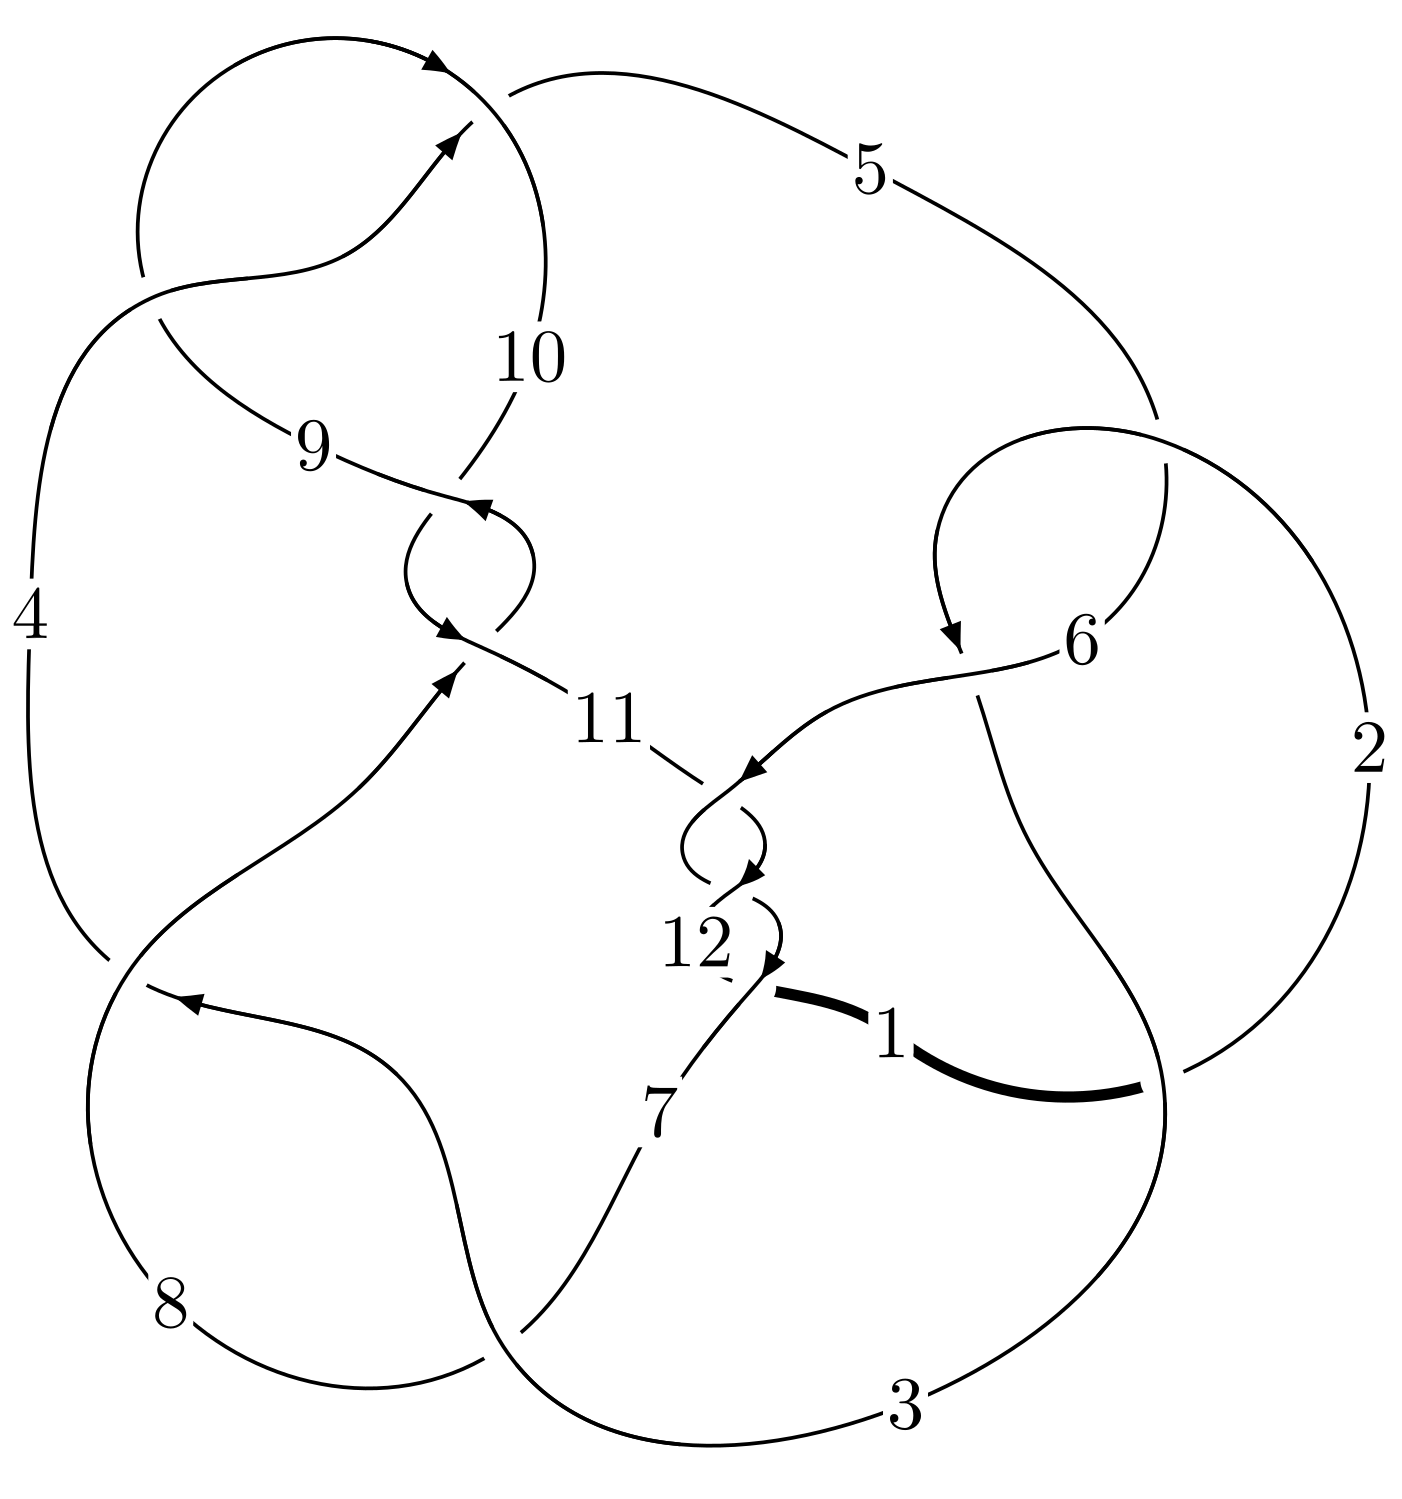
\includegraphics[width=112pt]{../../../GIT/diagram.site/Diagrams/png/2475_12n_0386.png}\\
\ \ \ A knot diagram\footnotemark}&
\allowdisplaybreaks
\textbf{Linearized knot diagam} \\
\cline{2-2}
 &
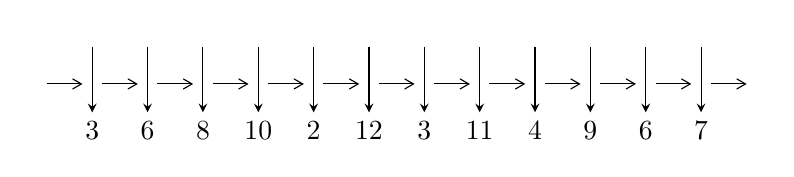
\begin{tikzpicture}[x=20pt, y=17pt]
	% nodes
	\node (C0) at (0, 0) {};
	\node (C1) at (1, 0) {};
	\node (C1U) at (1, +1) {};
	\node (C1D) at (1, -1) {3};

	\node (C2) at (2, 0) {};
	\node (C2U) at (2, +1) {};
	\node (C2D) at (2, -1) {6};

	\node (C3) at (3, 0) {};
	\node (C3U) at (3, +1) {};
	\node (C3D) at (3, -1) {8};

	\node (C4) at (4, 0) {};
	\node (C4U) at (4, +1) {};
	\node (C4D) at (4, -1) {10};

	\node (C5) at (5, 0) {};
	\node (C5U) at (5, +1) {};
	\node (C5D) at (5, -1) {2};

	\node (C6) at (6, 0) {};
	\node (C6U) at (6, +1) {};
	\node (C6D) at (6, -1) {12};

	\node (C7) at (7, 0) {};
	\node (C7U) at (7, +1) {};
	\node (C7D) at (7, -1) {3};

	\node (C8) at (8, 0) {};
	\node (C8U) at (8, +1) {};
	\node (C8D) at (8, -1) {11};

	\node (C9) at (9, 0) {};
	\node (C9U) at (9, +1) {};
	\node (C9D) at (9, -1) {4};

	\node (C10) at (10, 0) {};
	\node (C10U) at (10, +1) {};
	\node (C10D) at (10, -1) {9};

	\node (C11) at (11, 0) {};
	\node (C11U) at (11, +1) {};
	\node (C11D) at (11, -1) {6};

	\node (C12) at (12, 0) {};
	\node (C12U) at (12, +1) {};
	\node (C12D) at (12, -1) {7};
	\node (C13) at (13, 0) {};

	% arrows
	\draw[->,>={angle 60}]
	(C0) edge (C1) (C1) edge (C2) (C2) edge (C3) (C3) edge (C4) (C4) edge (C5) (C5) edge (C6) (C6) edge (C7) (C7) edge (C8) (C8) edge (C9) (C9) edge (C10) (C10) edge (C11) (C11) edge (C12) (C12) edge (C13) ;	\draw[->,>=stealth]
	(C1U) edge (C1D) (C2U) edge (C2D) (C3U) edge (C3D) (C4U) edge (C4D) (C5U) edge (C5D) (C6U) edge (C6D) (C7U) edge (C7D) (C8U) edge (C8D) (C9U) edge (C9D) (C10U) edge (C10D) (C11U) edge (C11D) (C12U) edge (C12D) ;
	\end{tikzpicture} \\
\hhline{~~} \\& 
\textbf{Solving Sequence} \\ \cline{2-2} 
 &
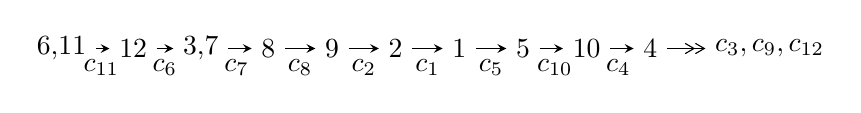
\begin{tikzpicture}[x=23pt, y=7pt]
	% node
	\node (A0) at (-1/8, 0) {6,11};
	\node (A1) at (1, 0) {12};
	\node (A2) at (33/16, 0) {3,7};
	\node (A3) at (25/8, 0) {8};
	\node (A4) at (33/8, 0) {9};
	\node (A5) at (41/8, 0) {2};
	\node (A6) at (49/8, 0) {1};
	\node (A7) at (57/8, 0) {5};
	\node (A8) at (65/8, 0) {10};
	\node (A9) at (73/8, 0) {4};
	\node (C1) at (1/2, -1) {$c_{11}$};
	\node (C2) at (3/2, -1) {$c_{6}$};
	\node (C3) at (21/8, -1) {$c_{7}$};
	\node (C4) at (29/8, -1) {$c_{8}$};
	\node (C5) at (37/8, -1) {$c_{2}$};
	\node (C6) at (45/8, -1) {$c_{1}$};
	\node (C7) at (53/8, -1) {$c_{5}$};
	\node (C8) at (61/8, -1) {$c_{10}$};
	\node (C9) at (69/8, -1) {$c_{4}$};
	\node (A10) at (11, 0) {$c_{3},c_{9},c_{12}$};

	% edge
	\draw[->,>=stealth]	
	(A0) edge (A1) (A1) edge (A2) (A2) edge (A3) (A3) edge (A4) (A4) edge (A5) (A5) edge (A6) (A6) edge (A7) (A7) edge (A8) (A8) edge (A9) ;
	\draw[->>,>={angle 60}]	
	(A9) edge (A10);
\end{tikzpicture} \\ 

\end{tabular} \\

\footnotetext{
The image of knot diagram is generated by the software ``\textbf{Draw programme}" developed by Andrew Bartholomew(\url{http://www.layer8.co.uk/maths/draw/index.htm\#Running-draw}), where we modified some parts for our purpose(\url{https://github.com/CATsTAILs/LinksPainter}).
}\phantom \\ \newline 
\centering \textbf{Ideals for irreducible components\footnotemark of $X_{\text{par}}$} 
 
\begin{align*}
I^u_{1}&=\langle 
u^{11}-3 u^{10}-13 u^9+39 u^8+46 u^7-146 u^6+10 u^5-54 u^4-15 u^3-91 u^2+32 b+3 u-1,\;a-1,\\
\phantom{I^u_{1}}&\phantom{= \langle  }u^{13}-3 u^{12}-14 u^{11}+42 u^{10}+59 u^9-185 u^8-36 u^7+92 u^6-25 u^5-5 u^4+18 u^3-6 u^2-3 u+1\rangle \\
I^u_{2}&=\langle 
b^4- b^2+2,\;a+1,\;u-1\rangle \\
I^u_{3}&=\langle 
b-1,\;a+1,\;u-1\rangle \\
I^u_{4}&=\langle 
b+1,\;a+1,\;u-1\rangle \\
I^u_{5}&=\langle 
b-1,\;a,\;u+1\rangle \\
I^u_{6}&=\langle 
b,\;a+1,\;u+1\rangle \\
I^u_{7}&=\langle 
b^4+1,\;a+1,\;u+1\rangle \\
\\
I^v_{1}&=\langle 
a,\;b-1,\;v-1\rangle \\
\end{align*}
\raggedright * 8 irreducible components of $\dim_{\mathbb{C}}=0$, with total 26 representations.\\
\footnotetext{All coefficients of polynomials are rational numbers. But the coefficients are sometimes approximated in decimal forms when there is not enough margin.}
\newpage
\renewcommand{\arraystretch}{1}
\centering \section*{I. $I^u_{1}= \langle u^{11}-3 u^{10}+\cdots+32 b-1,\;a-1,\;u^{13}-3 u^{12}+\cdots-3 u+1 \rangle$}
\flushleft \textbf{(i) Arc colorings}\\
\begin{tabular}{m{7pt} m{180pt} m{7pt} m{180pt} }
\flushright $a_{6}=$&$\begin{pmatrix}0\\u\end{pmatrix}$ \\
\flushright $a_{11}=$&$\begin{pmatrix}1\\0\end{pmatrix}$ \\
\flushright $a_{12}=$&$\begin{pmatrix}1\\u^2\end{pmatrix}$ \\
\flushright $a_{3}=$&$\begin{pmatrix}1\\-0.0312500 u^{11}+0.0937500 u^{10}+\cdots-0.0937500 u+0.0312500\end{pmatrix}$ \\
\flushright $a_{7}=$&$\begin{pmatrix}- u\\- u^3+u\end{pmatrix}$ \\
\flushright $a_{8}=$&$\begin{pmatrix}0.0312500 u^{12}-0.0937500 u^{11}+\cdots+0.0937500 u^{2}-2.03125 u\\\frac{7}{32} u^{12}-\frac{11}{16} u^{11}+\cdots+\frac{5}{8} u+\frac{1}{32}\end{pmatrix}$ \\
\flushright $a_{9}=$&$\begin{pmatrix}-0.187500 u^{12}+0.593750 u^{11}+\cdots-2.65625 u-0.0312500\\\frac{7}{32} u^{12}-\frac{11}{16} u^{11}+\cdots+\frac{5}{8} u+\frac{1}{32}\end{pmatrix}$ \\
\flushright $a_{2}=$&$\begin{pmatrix}1\\-0.0312500 u^{11}+0.0937500 u^{10}+\cdots-0.0937500 u+0.0312500\end{pmatrix}$ \\
\flushright $a_{1}=$&$\begin{pmatrix}- u^2+1\\- u^4+2 u^2\end{pmatrix}$ \\
\flushright $a_{5}=$&$\begin{pmatrix}u\\-0.0312500 u^{12}+0.0937500 u^{11}+\cdots-0.0937500 u^{2}+1.03125 u\end{pmatrix}$ \\
\flushright $a_{10}=$&$\begin{pmatrix}\frac{9}{16} u^{12}-\frac{31}{16} u^{11}+\cdots-4 u+2\\-0.812500 u^{12}+3.31250 u^{11}+\cdots+7.50000 u-2.06250\end{pmatrix}$ \\
\flushright $a_{4}=$&$\begin{pmatrix}-0.0312500 u^{12}+0.281250 u^{11}+\cdots+0.781250 u+0.750000\\-0.218750 u^{12}+1.09375 u^{11}+\cdots+2.71875 u-0.812500\end{pmatrix}$\\&\end{tabular}
\flushleft \textbf{(ii) Obstruction class $= -1$}\\~\\
\flushleft \textbf{(iii) Cusp Shapes $= -\frac{35}{16} u^{12}+\frac{145}{16} u^{11}+\frac{353}{16} u^{10}-\frac{1973}{16} u^9-\frac{21}{2} u^8+\frac{4023}{8} u^7-\frac{3425}{8} u^6-\frac{643}{8} u^5+\frac{3897}{16} u^4-\frac{2063}{16} u^3+\frac{161}{16} u^2+\frac{651}{16} u-\frac{231}{8}$}\\~\\
\newpage\renewcommand{\arraystretch}{1}
\flushleft \textbf{(iv) u-Polynomials at the component}\newline \\
\begin{tabular}{m{50pt}|m{274pt}}
Crossings & \hspace{64pt}u-Polynomials at each crossing \\
\hline $$\begin{aligned}c_{1}\end{aligned}$$&$\begin{aligned}
&u^{13}+37 u^{12}+\cdots+21 u+1
\end{aligned}$\\
\hline $$\begin{aligned}c_{2},c_{5},c_{6}\\c_{11},c_{12}\end{aligned}$$&$\begin{aligned}
&u^{13}+3 u^{12}+\cdots-3 u-1
\end{aligned}$\\
\hline $$\begin{aligned}c_{3},c_{7}\end{aligned}$$&$\begin{aligned}
&u^{13}-5 u^{12}+\cdots+36 u+26
\end{aligned}$\\
\hline $$\begin{aligned}c_{4},c_{9}\end{aligned}$$&$\begin{aligned}
&u^{13}+3 u^{12}+\cdots+8 u+2
\end{aligned}$\\
\hline $$\begin{aligned}c_{8},c_{10}\end{aligned}$$&$\begin{aligned}
&u^{13}+5 u^{12}+\cdots+32 u+4
\end{aligned}$\\
\hline
\end{tabular}\\~\\
\newpage\renewcommand{\arraystretch}{1}
\flushleft \textbf{(v) Riley Polynomials at the component}\newline \\
\begin{tabular}{m{50pt}|m{274pt}}
Crossings & \hspace{64pt}Riley Polynomials at each crossing \\
\hline $$\begin{aligned}c_{1}\end{aligned}$$&$\begin{aligned}
&y^{13}-237 y^{12}+\cdots+173 y-1
\end{aligned}$\\
\hline $$\begin{aligned}c_{2},c_{5},c_{6}\\c_{11},c_{12}\end{aligned}$$&$\begin{aligned}
&y^{13}-37 y^{12}+\cdots+21 y-1
\end{aligned}$\\
\hline $$\begin{aligned}c_{3},c_{7}\end{aligned}$$&$\begin{aligned}
&y^{13}-65 y^{12}+\cdots-5360 y-676
\end{aligned}$\\
\hline $$\begin{aligned}c_{4},c_{9}\end{aligned}$$&$\begin{aligned}
&y^{13}-5 y^{12}+\cdots+32 y-4
\end{aligned}$\\
\hline $$\begin{aligned}c_{8},c_{10}\end{aligned}$$&$\begin{aligned}
&y^{13}+7 y^{12}+\cdots+480 y-16
\end{aligned}$\\
\hline
\end{tabular}\\~\\
\newpage\flushleft \textbf{(vi) Complex Volumes and Cusp Shapes}
$$\begin{array}{c|c|c}  
\text{Solutions to }I^u_{1}& \I (\text{vol} + \sqrt{-1}CS) & \text{Cusp shape}\\
 \hline 
\begin{aligned}
u &= -0.584997 + 0.104914 I \\
a &= \phantom{-}1.00000\phantom{ +0.000000I} \\
b &= \phantom{-}1.224250 - 0.653734 I\end{aligned}
 & -0.88948 + 5.75156 I & -12.6714 - 7.2274 I \\ \hline\begin{aligned}
u &= -0.584997 - 0.104914 I \\
a &= \phantom{-}1.00000\phantom{ +0.000000I} \\
b &= \phantom{-}1.224250 + 0.653734 I\end{aligned}
 & -0.88948 - 5.75156 I & -12.6714 + 7.2274 I \\ \hline\begin{aligned}
u &= \phantom{-}0.140736 + 0.561263 I \\
a &= \phantom{-}1.00000\phantom{ +0.000000I} \\
b &= -0.773695 + 0.343562 I\end{aligned}
 & \phantom{-}1.39701 - 2.29590 I & -8.94612 + 4.81765 I \\ \hline\begin{aligned}
u &= \phantom{-}0.140736 - 0.561263 I \\
a &= \phantom{-}1.00000\phantom{ +0.000000I} \\
b &= -0.773695 - 0.343562 I\end{aligned}
 & \phantom{-}1.39701 + 2.29590 I & -8.94612 - 4.81765 I \\ \hline\begin{aligned}
u &= -0.571799\phantom{ +0.000000I} \\
a &= \phantom{-}1.00000\phantom{ +0.000000I} \\
b &= \phantom{-}1.29852\phantom{ +0.000000I}\end{aligned}
 & -4.92305\phantom{ +0.000000I} & -18.0630\phantom{ +0.000000I} \\ \hline\begin{aligned}
u &= \phantom{-}0.530717 + 0.126593 I \\
a &= \phantom{-}1.00000\phantom{ +0.000000I} \\
b &= \phantom{-}0.900850 + 0.616546 I\end{aligned}
 & \phantom{-}0.109607 - 0.527741 I & -11.42537 + 2.37191 I \\ \hline\begin{aligned}
u &= \phantom{-}0.530717 - 0.126593 I \\
a &= \phantom{-}1.00000\phantom{ +0.000000I} \\
b &= \phantom{-}0.900850 - 0.616546 I\end{aligned}
 & \phantom{-}0.109607 + 0.527741 I & -11.42537 - 2.37191 I \\ \hline\begin{aligned}
u &= \phantom{-}0.297204\phantom{ +0.000000I} \\
a &= \phantom{-}1.00000\phantom{ +0.000000I} \\
b &= \phantom{-}0.282107\phantom{ +0.000000I}\end{aligned}
 & -0.561817\phantom{ +0.000000I} & -17.7590\phantom{ +0.000000I} \\ \hline\begin{aligned}
u &= \phantom{-}2.49582 + 0.80059 I \\
a &= \phantom{-}1.00000\phantom{ +0.000000I} \\
b &= \phantom{-}3.34031 + 4.21214 I\end{aligned}
 & \phantom{-}16.3066 - 9.5421 I & -15.4017 + 4.1459 I \\ \hline\begin{aligned}
u &= \phantom{-}2.49582 - 0.80059 I \\
a &= \phantom{-}1.00000\phantom{ +0.000000I} \\
b &= \phantom{-}3.34031 - 4.21214 I\end{aligned}
 & \phantom{-}16.3066 + 9.5421 I & -15.4017 - 4.1459 I\\
 \hline 
 \end{array}$$\newpage$$\begin{array}{c|c|c}  
\text{Solutions to }I^u_{1}& \I (\text{vol} + \sqrt{-1}CS) & \text{Cusp shape}\\
 \hline 
\begin{aligned}
u &= -2.63506 + 0.50378 I \\
a &= \phantom{-}1.00000\phantom{ +0.000000I} \\
b &= \phantom{-}4.40111 - 2.78969 I\end{aligned}
 & \phantom{-}18.2542 + 3.1219 I & -13.76946 - 0.20883 I \\ \hline\begin{aligned}
u &= -2.63506 - 0.50378 I \\
a &= \phantom{-}1.00000\phantom{ +0.000000I} \\
b &= \phantom{-}4.40111 + 2.78969 I\end{aligned}
 & \phantom{-}18.2542 - 3.1219 I & -13.76946 + 0.20883 I \\ \hline\begin{aligned}
u &= \phantom{-}3.38017\phantom{ +0.000000I} \\
a &= \phantom{-}1.00000\phantom{ +0.000000I} \\
b &= \phantom{-}9.23373\phantom{ +0.000000I}\end{aligned}
 & \phantom{-}10.7959\phantom{ +0.000000I} & -17.7500\phantom{ +0.000000I}\\
 \hline 
 \end{array}$$\newpage\newpage\renewcommand{\arraystretch}{1}
\centering \section*{II. $I^u_{2}= \langle b^4- b^2+2,\;a+1,\;u-1 \rangle$}
\flushleft \textbf{(i) Arc colorings}\\
\begin{tabular}{m{7pt} m{180pt} m{7pt} m{180pt} }
\flushright $a_{6}=$&$\begin{pmatrix}0\\1\end{pmatrix}$ \\
\flushright $a_{11}=$&$\begin{pmatrix}1\\0\end{pmatrix}$ \\
\flushright $a_{12}=$&$\begin{pmatrix}1\\1\end{pmatrix}$ \\
\flushright $a_{3}=$&$\begin{pmatrix}-1\\b\end{pmatrix}$ \\
\flushright $a_{7}=$&$\begin{pmatrix}-1\\0\end{pmatrix}$ \\
\flushright $a_{8}=$&$\begin{pmatrix}b-1\\- b^2\end{pmatrix}$ \\
\flushright $a_{9}=$&$\begin{pmatrix}b^2+b-1\\- b^2\end{pmatrix}$ \\
\flushright $a_{2}=$&$\begin{pmatrix}-1\\b+1\end{pmatrix}$ \\
\flushright $a_{1}=$&$\begin{pmatrix}0\\1\end{pmatrix}$ \\
\flushright $a_{5}=$&$\begin{pmatrix}1\\- b\end{pmatrix}$ \\
\flushright $a_{10}=$&$\begin{pmatrix}b^3-1\\- b^2+2\end{pmatrix}$ \\
\flushright $a_{4}=$&$\begin{pmatrix}b^2- b-1\\- b^3+b\end{pmatrix}$\\&\end{tabular}
\flushleft \textbf{(ii) Obstruction class $= 1$}\\~\\
\flushleft \textbf{(iii) Cusp Shapes $= 4 b^2-20$}\\~\\
\newpage\renewcommand{\arraystretch}{1}
\flushleft \textbf{(iv) u-Polynomials at the component}\newline \\
\begin{tabular}{m{50pt}|m{274pt}}
Crossings & \hspace{64pt}u-Polynomials at each crossing \\
\hline $$\begin{aligned}c_{1},c_{5},c_{11}\\c_{12}\end{aligned}$$&$\begin{aligned}
&(u-1)^4
\end{aligned}$\\
\hline $$\begin{aligned}c_{2},c_{6}\end{aligned}$$&$\begin{aligned}
&(u+1)^4
\end{aligned}$\\
\hline $$\begin{aligned}c_{3},c_{4},c_{7}\\c_{9}\end{aligned}$$&$\begin{aligned}
&u^4- u^2+2
\end{aligned}$\\
\hline $$\begin{aligned}c_{8}\end{aligned}$$&$\begin{aligned}
&(u^2- u+2)^2
\end{aligned}$\\
\hline $$\begin{aligned}c_{10}\end{aligned}$$&$\begin{aligned}
&(u^2+u+2)^2
\end{aligned}$\\
\hline
\end{tabular}\\~\\
\newpage\renewcommand{\arraystretch}{1}
\flushleft \textbf{(v) Riley Polynomials at the component}\newline \\
\begin{tabular}{m{50pt}|m{274pt}}
Crossings & \hspace{64pt}Riley Polynomials at each crossing \\
\hline $$\begin{aligned}c_{1},c_{2},c_{5}\\c_{6},c_{11},c_{12}\end{aligned}$$&$\begin{aligned}
&(y-1)^4
\end{aligned}$\\
\hline $$\begin{aligned}c_{3},c_{4},c_{7}\\c_{9}\end{aligned}$$&$\begin{aligned}
&(y^2- y+2)^2
\end{aligned}$\\
\hline $$\begin{aligned}c_{8},c_{10}\end{aligned}$$&$\begin{aligned}
&(y^2+3 y+4)^2
\end{aligned}$\\
\hline
\end{tabular}\\~\\
\newpage\flushleft \textbf{(vi) Complex Volumes and Cusp Shapes}
$$\begin{array}{c|c|c}  
\text{Solutions to }I^u_{2}& \I (\text{vol} + \sqrt{-1}CS) & \text{Cusp shape}\\
 \hline 
\begin{aligned}
u &= \phantom{-}1.00000\phantom{ +0.000000I} \\
a &= -1.00000\phantom{ +0.000000I} \\
b &= \phantom{-}0.978318 + 0.676097 I\end{aligned}
 & -2.46740 - 5.33349 I & -18.0000 + 5.2915 I \\ \hline\begin{aligned}
u &= \phantom{-}1.00000\phantom{ +0.000000I} \\
a &= -1.00000\phantom{ +0.000000I} \\
b &= \phantom{-}0.978318 - 0.676097 I\end{aligned}
 & -2.46740 + 5.33349 I & -18.0000 - 5.2915 I \\ \hline\begin{aligned}
u &= \phantom{-}1.00000\phantom{ +0.000000I} \\
a &= -1.00000\phantom{ +0.000000I} \\
b &= -0.978318 + 0.676097 I\end{aligned}
 & -2.46740 + 5.33349 I & -18.0000 - 5.2915 I \\ \hline\begin{aligned}
u &= \phantom{-}1.00000\phantom{ +0.000000I} \\
a &= -1.00000\phantom{ +0.000000I} \\
b &= -0.978318 - 0.676097 I\end{aligned}
 & -2.46740 - 5.33349 I & -18.0000 + 5.2915 I\\
 \hline 
 \end{array}$$\newpage\newpage\renewcommand{\arraystretch}{1}
\centering \section*{III. $I^u_{3}= \langle b-1,\;a+1,\;u-1 \rangle$}
\flushleft \textbf{(i) Arc colorings}\\
\begin{tabular}{m{7pt} m{180pt} m{7pt} m{180pt} }
\flushright $a_{6}=$&$\begin{pmatrix}0\\1\end{pmatrix}$ \\
\flushright $a_{11}=$&$\begin{pmatrix}1\\0\end{pmatrix}$ \\
\flushright $a_{12}=$&$\begin{pmatrix}1\\1\end{pmatrix}$ \\
\flushright $a_{3}=$&$\begin{pmatrix}-1\\1\end{pmatrix}$ \\
\flushright $a_{7}=$&$\begin{pmatrix}-1\\0\end{pmatrix}$ \\
\flushright $a_{8}=$&$\begin{pmatrix}0\\-1\end{pmatrix}$ \\
\flushright $a_{9}=$&$\begin{pmatrix}1\\-1\end{pmatrix}$ \\
\flushright $a_{2}=$&$\begin{pmatrix}-1\\2\end{pmatrix}$ \\
\flushright $a_{1}=$&$\begin{pmatrix}0\\1\end{pmatrix}$ \\
\flushright $a_{5}=$&$\begin{pmatrix}1\\-1\end{pmatrix}$ \\
\flushright $a_{10}=$&$\begin{pmatrix}2\\-1\end{pmatrix}$ \\
\flushright $a_{4}=$&$\begin{pmatrix}-1\\0\end{pmatrix}$\\&\end{tabular}
\flushleft \textbf{(ii) Obstruction class $= 1$}\\~\\
\flushleft \textbf{(iii) Cusp Shapes $= -24$}\\~\\
\newpage\renewcommand{\arraystretch}{1}
\flushleft \textbf{(iv) u-Polynomials at the component}\newline \\
\begin{tabular}{m{50pt}|m{274pt}}
Crossings & \hspace{64pt}u-Polynomials at each crossing \\
\hline $$\begin{aligned}c_{1},c_{3},c_{4}\\c_{5},c_{8},c_{11}\\c_{12}\end{aligned}$$&$\begin{aligned}
&u-1
\end{aligned}$\\
\hline $$\begin{aligned}c_{2},c_{6},c_{7}\\c_{9},c_{10}\end{aligned}$$&$\begin{aligned}
&u+1
\end{aligned}$\\
\hline
\end{tabular}\\~\\
\newpage\renewcommand{\arraystretch}{1}
\flushleft \textbf{(v) Riley Polynomials at the component}\newline \\
\begin{tabular}{m{50pt}|m{274pt}}
Crossings & \hspace{64pt}Riley Polynomials at each crossing \\
\hline $$\begin{aligned}c_{1},c_{2},c_{3}\\c_{4},c_{5},c_{6}\\c_{7},c_{8},c_{9}\\c_{10},c_{11},c_{12}\end{aligned}$$&$\begin{aligned}
&y-1
\end{aligned}$\\
\hline
\end{tabular}\\~\\
\newpage\flushleft \textbf{(vi) Complex Volumes and Cusp Shapes}
$$\begin{array}{c|c|c}  
\text{Solutions to }I^u_{3}& \I (\text{vol} + \sqrt{-1}CS) & \text{Cusp shape}\\
 \hline 
\begin{aligned}
u &= \phantom{-}1.00000\phantom{ +0.000000I} \\
a &= -1.00000\phantom{ +0.000000I} \\
b &= \phantom{-}1.00000\phantom{ +0.000000I}\end{aligned}
 & -6.57974\phantom{ +0.000000I} & -24.0000\phantom{ +0.000000I}\\
 \hline 
 \end{array}$$\newpage\newpage\renewcommand{\arraystretch}{1}
\centering \section*{IV. $I^u_{4}= \langle b+1,\;a+1,\;u-1 \rangle$}
\flushleft \textbf{(i) Arc colorings}\\
\begin{tabular}{m{7pt} m{180pt} m{7pt} m{180pt} }
\flushright $a_{6}=$&$\begin{pmatrix}0\\1\end{pmatrix}$ \\
\flushright $a_{11}=$&$\begin{pmatrix}1\\0\end{pmatrix}$ \\
\flushright $a_{12}=$&$\begin{pmatrix}1\\1\end{pmatrix}$ \\
\flushright $a_{3}=$&$\begin{pmatrix}-1\\-1\end{pmatrix}$ \\
\flushright $a_{7}=$&$\begin{pmatrix}-1\\0\end{pmatrix}$ \\
\flushright $a_{8}=$&$\begin{pmatrix}-2\\-1\end{pmatrix}$ \\
\flushright $a_{9}=$&$\begin{pmatrix}-1\\-1\end{pmatrix}$ \\
\flushright $a_{2}=$&$\begin{pmatrix}-1\\0\end{pmatrix}$ \\
\flushright $a_{1}=$&$\begin{pmatrix}0\\1\end{pmatrix}$ \\
\flushright $a_{5}=$&$\begin{pmatrix}1\\1\end{pmatrix}$ \\
\flushright $a_{10}=$&$\begin{pmatrix}0\\-1\end{pmatrix}$ \\
\flushright $a_{4}=$&$\begin{pmatrix}1\\0\end{pmatrix}$\\&\end{tabular}
\flushleft \textbf{(ii) Obstruction class $= 1$}\\~\\
\flushleft \textbf{(iii) Cusp Shapes $= -24$}\\~\\
\newpage\renewcommand{\arraystretch}{1}
\flushleft \textbf{(iv) u-Polynomials at the component}\newline \\
\begin{tabular}{m{50pt}|m{274pt}}
Crossings & \hspace{64pt}u-Polynomials at each crossing \\
\hline $$\begin{aligned}c_{1},c_{5},c_{7}\\c_{8},c_{9},c_{11}\\c_{12}\end{aligned}$$&$\begin{aligned}
&u-1
\end{aligned}$\\
\hline $$\begin{aligned}c_{2},c_{3},c_{4}\\c_{6},c_{10}\end{aligned}$$&$\begin{aligned}
&u+1
\end{aligned}$\\
\hline
\end{tabular}\\~\\
\newpage\renewcommand{\arraystretch}{1}
\flushleft \textbf{(v) Riley Polynomials at the component}\newline \\
\begin{tabular}{m{50pt}|m{274pt}}
Crossings & \hspace{64pt}Riley Polynomials at each crossing \\
\hline $$\begin{aligned}c_{1},c_{2},c_{3}\\c_{4},c_{5},c_{6}\\c_{7},c_{8},c_{9}\\c_{10},c_{11},c_{12}\end{aligned}$$&$\begin{aligned}
&y-1
\end{aligned}$\\
\hline
\end{tabular}\\~\\
\newpage\flushleft \textbf{(vi) Complex Volumes and Cusp Shapes}
$$\begin{array}{c|c|c}  
\text{Solutions to }I^u_{4}& \I (\text{vol} + \sqrt{-1}CS) & \text{Cusp shape}\\
 \hline 
\begin{aligned}
u &= \phantom{-}1.00000\phantom{ +0.000000I} \\
a &= -1.00000\phantom{ +0.000000I} \\
b &= -1.00000\phantom{ +0.000000I}\end{aligned}
 & -6.57974\phantom{ +0.000000I} & -24.0000\phantom{ +0.000000I}\\
 \hline 
 \end{array}$$\newpage\newpage\renewcommand{\arraystretch}{1}
\centering \section*{V. $I^u_{5}= \langle b-1,\;a,\;u+1 \rangle$}
\flushleft \textbf{(i) Arc colorings}\\
\begin{tabular}{m{7pt} m{180pt} m{7pt} m{180pt} }
\flushright $a_{6}=$&$\begin{pmatrix}0\\-1\end{pmatrix}$ \\
\flushright $a_{11}=$&$\begin{pmatrix}1\\0\end{pmatrix}$ \\
\flushright $a_{12}=$&$\begin{pmatrix}1\\1\end{pmatrix}$ \\
\flushright $a_{3}=$&$\begin{pmatrix}0\\1\end{pmatrix}$ \\
\flushright $a_{7}=$&$\begin{pmatrix}1\\0\end{pmatrix}$ \\
\flushright $a_{8}=$&$\begin{pmatrix}1\\1\end{pmatrix}$ \\
\flushright $a_{9}=$&$\begin{pmatrix}0\\1\end{pmatrix}$ \\
\flushright $a_{2}=$&$\begin{pmatrix}0\\1\end{pmatrix}$ \\
\flushright $a_{1}=$&$\begin{pmatrix}0\\1\end{pmatrix}$ \\
\flushright $a_{5}=$&$\begin{pmatrix}0\\-1\end{pmatrix}$ \\
\flushright $a_{10}=$&$\begin{pmatrix}1\\-1\end{pmatrix}$ \\
\flushright $a_{4}=$&$\begin{pmatrix}-1\\0\end{pmatrix}$\\&\end{tabular}
\flushleft \textbf{(ii) Obstruction class $= -1$}\\~\\
\flushleft \textbf{(iii) Cusp Shapes $= -18$}\\~\\
\newpage\renewcommand{\arraystretch}{1}
\flushleft \textbf{(iv) u-Polynomials at the component}\newline \\
\begin{tabular}{m{50pt}|m{274pt}}
Crossings & \hspace{64pt}u-Polynomials at each crossing \\
\hline $$\begin{aligned}c_{1},c_{2},c_{5}\end{aligned}$$&$\begin{aligned}
&u
\end{aligned}$\\
\hline $$\begin{aligned}c_{3},c_{4},c_{6}\\c_{7},c_{9},c_{11}\\c_{12}\end{aligned}$$&$\begin{aligned}
&u-1
\end{aligned}$\\
\hline $$\begin{aligned}c_{8},c_{10}\end{aligned}$$&$\begin{aligned}
&u+1
\end{aligned}$\\
\hline
\end{tabular}\\~\\
\newpage\renewcommand{\arraystretch}{1}
\flushleft \textbf{(v) Riley Polynomials at the component}\newline \\
\begin{tabular}{m{50pt}|m{274pt}}
Crossings & \hspace{64pt}Riley Polynomials at each crossing \\
\hline $$\begin{aligned}c_{1},c_{2},c_{5}\end{aligned}$$&$\begin{aligned}
&y
\end{aligned}$\\
\hline $$\begin{aligned}c_{3},c_{4},c_{6}\\c_{7},c_{8},c_{9}\\c_{10},c_{11},c_{12}\end{aligned}$$&$\begin{aligned}
&y-1
\end{aligned}$\\
\hline
\end{tabular}\\~\\
\newpage\flushleft \textbf{(vi) Complex Volumes and Cusp Shapes}
$$\begin{array}{c|c|c}  
\text{Solutions to }I^u_{5}& \I (\text{vol} + \sqrt{-1}CS) & \text{Cusp shape}\\
 \hline 
\begin{aligned}
u &= -1.00000\phantom{ +0.000000I} \\
a &= \phantom{-0.000000 } 0 \\
b &= \phantom{-}1.00000\phantom{ +0.000000I}\end{aligned}
 & -4.93480\phantom{ +0.000000I} & -18.0000\phantom{ +0.000000I}\\
 \hline 
 \end{array}$$\newpage\newpage\renewcommand{\arraystretch}{1}
\centering \section*{VI. $I^u_{6}= \langle b,\;a+1,\;u+1 \rangle$}
\flushleft \textbf{(i) Arc colorings}\\
\begin{tabular}{m{7pt} m{180pt} m{7pt} m{180pt} }
\flushright $a_{6}=$&$\begin{pmatrix}0\\-1\end{pmatrix}$ \\
\flushright $a_{11}=$&$\begin{pmatrix}1\\0\end{pmatrix}$ \\
\flushright $a_{12}=$&$\begin{pmatrix}1\\1\end{pmatrix}$ \\
\flushright $a_{3}=$&$\begin{pmatrix}-1\\0\end{pmatrix}$ \\
\flushright $a_{7}=$&$\begin{pmatrix}1\\0\end{pmatrix}$ \\
\flushright $a_{8}=$&$\begin{pmatrix}1\\0\end{pmatrix}$ \\
\flushright $a_{9}=$&$\begin{pmatrix}1\\0\end{pmatrix}$ \\
\flushright $a_{2}=$&$\begin{pmatrix}-1\\1\end{pmatrix}$ \\
\flushright $a_{1}=$&$\begin{pmatrix}0\\1\end{pmatrix}$ \\
\flushright $a_{5}=$&$\begin{pmatrix}-1\\0\end{pmatrix}$ \\
\flushright $a_{10}=$&$\begin{pmatrix}1\\0\end{pmatrix}$ \\
\flushright $a_{4}=$&$\begin{pmatrix}-1\\0\end{pmatrix}$\\&\end{tabular}
\flushleft \textbf{(ii) Obstruction class $= 1$}\\~\\
\flushleft \textbf{(iii) Cusp Shapes $= -12$}\\~\\
\newpage\renewcommand{\arraystretch}{1}
\flushleft \textbf{(iv) u-Polynomials at the component}\newline \\
\begin{tabular}{m{50pt}|m{274pt}}
Crossings & \hspace{64pt}u-Polynomials at each crossing \\
\hline $$\begin{aligned}c_{1},c_{2},c_{6}\end{aligned}$$&$\begin{aligned}
&u-1
\end{aligned}$\\
\hline $$\begin{aligned}c_{3},c_{4},c_{7}\\c_{8},c_{9},c_{10}\end{aligned}$$&$\begin{aligned}
&u
\end{aligned}$\\
\hline $$\begin{aligned}c_{5},c_{11},c_{12}\end{aligned}$$&$\begin{aligned}
&u+1
\end{aligned}$\\
\hline
\end{tabular}\\~\\
\newpage\renewcommand{\arraystretch}{1}
\flushleft \textbf{(v) Riley Polynomials at the component}\newline \\
\begin{tabular}{m{50pt}|m{274pt}}
Crossings & \hspace{64pt}Riley Polynomials at each crossing \\
\hline $$\begin{aligned}c_{1},c_{2},c_{5}\\c_{6},c_{11},c_{12}\end{aligned}$$&$\begin{aligned}
&y-1
\end{aligned}$\\
\hline $$\begin{aligned}c_{3},c_{4},c_{7}\\c_{8},c_{9},c_{10}\end{aligned}$$&$\begin{aligned}
&y
\end{aligned}$\\
\hline
\end{tabular}\\~\\
\newpage\flushleft \textbf{(vi) Complex Volumes and Cusp Shapes}
$$\begin{array}{c|c|c}  
\text{Solutions to }I^u_{6}& \I (\text{vol} + \sqrt{-1}CS) & \text{Cusp shape}\\
 \hline 
\begin{aligned}
u &= -1.00000\phantom{ +0.000000I} \\
a &= -1.00000\phantom{ +0.000000I} \\
b &= \phantom{-0.000000 } 0\end{aligned}
 & -3.28987\phantom{ +0.000000I} & -12.0000\phantom{ +0.000000I}\\
 \hline 
 \end{array}$$\newpage\newpage\renewcommand{\arraystretch}{1}
\centering \section*{VII. $I^u_{7}= \langle b^4+1,\;a+1,\;u+1 \rangle$}
\flushleft \textbf{(i) Arc colorings}\\
\begin{tabular}{m{7pt} m{180pt} m{7pt} m{180pt} }
\flushright $a_{6}=$&$\begin{pmatrix}0\\-1\end{pmatrix}$ \\
\flushright $a_{11}=$&$\begin{pmatrix}1\\0\end{pmatrix}$ \\
\flushright $a_{12}=$&$\begin{pmatrix}1\\1\end{pmatrix}$ \\
\flushright $a_{3}=$&$\begin{pmatrix}-1\\b\end{pmatrix}$ \\
\flushright $a_{7}=$&$\begin{pmatrix}1\\0\end{pmatrix}$ \\
\flushright $a_{8}=$&$\begin{pmatrix}- b+1\\b^2\end{pmatrix}$ \\
\flushright $a_{9}=$&$\begin{pmatrix}- b^2- b+1\\b^2\end{pmatrix}$ \\
\flushright $a_{2}=$&$\begin{pmatrix}-1\\b+1\end{pmatrix}$ \\
\flushright $a_{1}=$&$\begin{pmatrix}0\\1\end{pmatrix}$ \\
\flushright $a_{5}=$&$\begin{pmatrix}-1\\b\end{pmatrix}$ \\
\flushright $a_{10}=$&$\begin{pmatrix}b^3- b^2\\1\end{pmatrix}$ \\
\flushright $a_{4}=$&$\begin{pmatrix}b^2- b-1\\- b^3+b\end{pmatrix}$\\&\end{tabular}
\flushleft \textbf{(ii) Obstruction class $= 1$}\\~\\
\flushleft \textbf{(iii) Cusp Shapes $= -16$}\\~\\
\newpage\renewcommand{\arraystretch}{1}
\flushleft \textbf{(iv) u-Polynomials at the component}\newline \\
\begin{tabular}{m{50pt}|m{274pt}}
Crossings & \hspace{64pt}u-Polynomials at each crossing \\
\hline $$\begin{aligned}c_{1},c_{2},c_{6}\end{aligned}$$&$\begin{aligned}
&(u-1)^4
\end{aligned}$\\
\hline $$\begin{aligned}c_{3},c_{4},c_{7}\\c_{9}\end{aligned}$$&$\begin{aligned}
&u^4+1
\end{aligned}$\\
\hline $$\begin{aligned}c_{5},c_{11},c_{12}\end{aligned}$$&$\begin{aligned}
&(u+1)^4
\end{aligned}$\\
\hline $$\begin{aligned}c_{8},c_{10}\end{aligned}$$&$\begin{aligned}
&(u^2+1)^2
\end{aligned}$\\
\hline
\end{tabular}\\~\\
\newpage\renewcommand{\arraystretch}{1}
\flushleft \textbf{(v) Riley Polynomials at the component}\newline \\
\begin{tabular}{m{50pt}|m{274pt}}
Crossings & \hspace{64pt}Riley Polynomials at each crossing \\
\hline $$\begin{aligned}c_{1},c_{2},c_{5}\\c_{6},c_{11},c_{12}\end{aligned}$$&$\begin{aligned}
&(y-1)^4
\end{aligned}$\\
\hline $$\begin{aligned}c_{3},c_{4},c_{7}\\c_{9}\end{aligned}$$&$\begin{aligned}
&(y^2+1)^2
\end{aligned}$\\
\hline $$\begin{aligned}c_{8},c_{10}\end{aligned}$$&$\begin{aligned}
&(y+1)^4
\end{aligned}$\\
\hline
\end{tabular}\\~\\
\newpage\flushleft \textbf{(vi) Complex Volumes and Cusp Shapes}
$$\begin{array}{c|c|c}  
\text{Solutions to }I^u_{7}& \I (\text{vol} + \sqrt{-1}CS) & \text{Cusp shape}\\
 \hline 
\begin{aligned}
u &= -1.00000\phantom{ +0.000000I} \\
a &= -1.00000\phantom{ +0.000000I} \\
b &= \phantom{-}0.707107 + 0.707107 I\end{aligned}
 & -1.64493\phantom{ +0.000000I} & -16.0000\phantom{ +0.000000I} \\ \hline\begin{aligned}
u &= -1.00000\phantom{ +0.000000I} \\
a &= -1.00000\phantom{ +0.000000I} \\
b &= \phantom{-}0.707107 - 0.707107 I\end{aligned}
 & -1.64493\phantom{ +0.000000I} & -16.0000\phantom{ +0.000000I} \\ \hline\begin{aligned}
u &= -1.00000\phantom{ +0.000000I} \\
a &= -1.00000\phantom{ +0.000000I} \\
b &= -0.707107 + 0.707107 I\end{aligned}
 & -1.64493\phantom{ +0.000000I} & -16.0000\phantom{ +0.000000I} \\ \hline\begin{aligned}
u &= -1.00000\phantom{ +0.000000I} \\
a &= -1.00000\phantom{ +0.000000I} \\
b &= -0.707107 - 0.707107 I\end{aligned}
 & -1.64493\phantom{ +0.000000I} & -16.0000\phantom{ +0.000000I}\\
 \hline 
 \end{array}$$\newpage\newpage\renewcommand{\arraystretch}{1}
\centering \section*{VIII. $I^v_{1}= \langle a,\;b-1,\;v-1 \rangle$}
\flushleft \textbf{(i) Arc colorings}\\
\begin{tabular}{m{7pt} m{180pt} m{7pt} m{180pt} }
\flushright $a_{6}=$&$\begin{pmatrix}1\\0\end{pmatrix}$ \\
\flushright $a_{11}=$&$\begin{pmatrix}1\\0\end{pmatrix}$ \\
\flushright $a_{12}=$&$\begin{pmatrix}1\\0\end{pmatrix}$ \\
\flushright $a_{3}=$&$\begin{pmatrix}0\\1\end{pmatrix}$ \\
\flushright $a_{7}=$&$\begin{pmatrix}1\\0\end{pmatrix}$ \\
\flushright $a_{8}=$&$\begin{pmatrix}1\\1\end{pmatrix}$ \\
\flushright $a_{9}=$&$\begin{pmatrix}0\\1\end{pmatrix}$ \\
\flushright $a_{2}=$&$\begin{pmatrix}1\\1\end{pmatrix}$ \\
\flushright $a_{1}=$&$\begin{pmatrix}1\\0\end{pmatrix}$ \\
\flushright $a_{5}=$&$\begin{pmatrix}0\\-1\end{pmatrix}$ \\
\flushright $a_{10}=$&$\begin{pmatrix}1\\-1\end{pmatrix}$ \\
\flushright $a_{4}=$&$\begin{pmatrix}-1\\0\end{pmatrix}$\\&\end{tabular}
\flushleft \textbf{(ii) Obstruction class $= -1$}\\~\\
\flushleft \textbf{(iii) Cusp Shapes $= -18$}\\~\\
\newpage\renewcommand{\arraystretch}{1}
\flushleft \textbf{(iv) u-Polynomials at the component}\newline \\
\begin{tabular}{m{50pt}|m{274pt}}
Crossings & \hspace{64pt}u-Polynomials at each crossing \\
\hline $$\begin{aligned}c_{1},c_{8},c_{10}\end{aligned}$$&$\begin{aligned}
&u+1
\end{aligned}$\\
\hline $$\begin{aligned}c_{2},c_{3},c_{4}\\c_{5},c_{7},c_{9}\end{aligned}$$&$\begin{aligned}
&u-1
\end{aligned}$\\
\hline $$\begin{aligned}c_{6},c_{11},c_{12}\end{aligned}$$&$\begin{aligned}
&u
\end{aligned}$\\
\hline
\end{tabular}\\~\\
\newpage\renewcommand{\arraystretch}{1}
\flushleft \textbf{(v) Riley Polynomials at the component}\newline \\
\begin{tabular}{m{50pt}|m{274pt}}
Crossings & \hspace{64pt}Riley Polynomials at each crossing \\
\hline $$\begin{aligned}c_{1},c_{2},c_{3}\\c_{4},c_{5},c_{7}\\c_{8},c_{9},c_{10}\end{aligned}$$&$\begin{aligned}
&y-1
\end{aligned}$\\
\hline $$\begin{aligned}c_{6},c_{11},c_{12}\end{aligned}$$&$\begin{aligned}
&y
\end{aligned}$\\
\hline
\end{tabular}\\~\\
\newpage\flushleft \textbf{(vi) Complex Volumes and Cusp Shapes}
$$\begin{array}{c|c|c}  
\text{Solutions to }I^v_{1}& \I (\text{vol} + \sqrt{-1}CS) & \text{Cusp shape}\\
 \hline 
\begin{aligned}
v &= \phantom{-}1.00000\phantom{ +0.000000I} \\
a &= \phantom{-0.000000 } 0 \\
b &= \phantom{-}1.00000\phantom{ +0.000000I}\end{aligned}
 & -4.93480\phantom{ +0.000000I} & -18.0000\phantom{ +0.000000I}\\
 \hline 
 \end{array}$$\newpage
\newpage\renewcommand{\arraystretch}{1}
\centering \section*{ IX. u-Polynomials}
\begin{tabular}{m{50pt}|m{274pt}}
Crossings & \hspace{64pt}u-Polynomials at each crossing \\
\hline $$\begin{aligned}c_{1}\end{aligned}$$&$\begin{aligned}
&u(u-1)^{11}(u+1)(u^{13}+37 u^{12}+\cdots+21 u+1)
\end{aligned}$\\
\hline $$\begin{aligned}c_{2},c_{6}\end{aligned}$$&$\begin{aligned}
&u(u-1)^6(u+1)^6(u^{13}+3 u^{12}+\cdots-3 u-1)
\end{aligned}$\\
\hline $$\begin{aligned}c_{3},c_{7}\end{aligned}$$&$\begin{aligned}
&u(u-1)^3(u+1)(u^4+1)(u^4- u^2+2)(u^{13}-5 u^{12}+\cdots+36 u+26)
\end{aligned}$\\
\hline $$\begin{aligned}c_{4},c_{9}\end{aligned}$$&$\begin{aligned}
&u(u-1)^3(u+1)(u^4+1)(u^4- u^2+2)(u^{13}+3 u^{12}+\cdots+8 u+2)
\end{aligned}$\\
\hline $$\begin{aligned}c_{5},c_{11},c_{12}\end{aligned}$$&$\begin{aligned}
&u(u-1)^7(u+1)^5(u^{13}+3 u^{12}+\cdots-3 u-1)
\end{aligned}$\\
\hline $$\begin{aligned}c_{8}\end{aligned}$$&$\begin{aligned}
&u(u-1)^2(u+1)^2(u^2+1)^2(u^2- u+2)^{2}(u^{13}+5 u^{12}+\cdots+32 u+4)
\end{aligned}$\\
\hline $$\begin{aligned}c_{10}\end{aligned}$$&$\begin{aligned}
&u(u+1)^4(u^2+1)^2(u^2+u+2)^2(u^{13}+5 u^{12}+\cdots+32 u+4)
\end{aligned}$\\
\hline
\end{tabular}\newpage\renewcommand{\arraystretch}{1}
\centering \section*{ X. Riley Polynomials}
\begin{tabular}{m{50pt}|m{274pt}}
Crossings & \hspace{64pt}Riley Polynomials at each crossing \\
\hline $$\begin{aligned}c_{1}\end{aligned}$$&$\begin{aligned}
&y(y-1)^{12}(y^{13}-237 y^{12}+\cdots+173 y-1)
\end{aligned}$\\
\hline $$\begin{aligned}c_{2},c_{5},c_{6}\\c_{11},c_{12}\end{aligned}$$&$\begin{aligned}
&y(y-1)^{12}(y^{13}-37 y^{12}+\cdots+21 y-1)
\end{aligned}$\\
\hline $$\begin{aligned}c_{3},c_{7}\end{aligned}$$&$\begin{aligned}
&y(y-1)^4(y^2+1)^2(y^2- y+2)^2(y^{13}-65 y^{12}+\cdots-5360 y-676)
\end{aligned}$\\
\hline $$\begin{aligned}c_{4},c_{9}\end{aligned}$$&$\begin{aligned}
&y(y-1)^4(y^2+1)^2(y^2- y+2)^2(y^{13}-5 y^{12}+\cdots+32 y-4)
\end{aligned}$\\
\hline $$\begin{aligned}c_{8},c_{10}\end{aligned}$$&$\begin{aligned}
&y(y-1)^4(y+1)^4(y^2+3 y+4)^{2}(y^{13}+7 y^{12}+\cdots+480 y-16)
\end{aligned}$\\
\hline
\end{tabular}
\vskip 2pc
\end{document}